% ─────────────────────────────────────────────────────────────
% ACTIVIDAD 4: Heurísticas para la tasa de aprendizaje
% ─────────────────────────────────────────────────────────────

La tasa de aprendizaje ($\eta$) es uno de los hiperparámetros más críticos en el entrenamiento de redes neuronales mediante retropropagación. Un valor excesivamente grande provoca oscilaciones y divergencia; uno demasiado pequeño ralentiza la convergencia o atrapa el optimizador en mínimos locales. A continuación se presentan tres heurísticas ampliamente adoptadas.

% ─────────────────────────────────────────────────────────────
\subsection{Heurística 1: Decaimiento de la tasa de aprendizaje}
% ─────────────────────────────────────────────────────────────

Consiste en reducir progresivamente $\eta$ a medida que avanzan las épocas. La idea central es permitir pasos grandes al inicio (exploración rápida del espacio de pesos) y pasos pequeños al final (refinamiento cercano al óptimo).

\textbf{Formulación matemática.} Dos variantes clásicas son:

\begin{enumerate}[label=\arabic*.]
    \item \textbf{Decaimiento exponencial:}
    \begin{equation}
        \eta(t) = \eta_0 \cdot e^{-\lambda t},
    \end{equation}
    donde $\eta_0$ es la tasa inicial, $\lambda > 0$ es la tasa de decaimiento y $t$ es el número de época.

    \item \textbf{Decaimiento por etapas (step decay):}
    \begin{equation}
        \eta(t) = \eta_0 \cdot \gamma^{\lfloor t / s \rfloor},
    \end{equation}
    donde $\gamma \in (0,1)$ es el factor de reducción y $s$ es el período (cada cuántas épocas se reduce la tasa).
\end{enumerate}

% ─────────────────────────────────────────────────────────────
\subsection{Heurística 2: Tasa de aprendizaje adaptativa (escalamiento por coordenadas)}
% ─────────────────────────────────────────────────────────────

En lugar de usar una tasa global, se adapta una tasa independiente para cada parámetro (peso) según la historia de sus gradientes. Este principio subyace en algoritmos como AdaGrad, RMSprop y Adam.

\textbf{Formulación de AdaGrad.} Sea $g_{t,i}$ el gradiente del parámetro $i$ en la época $t$. Se acumula el cuadrado del gradiente:
\begin{equation}
    G_{t,i} = G_{t-1,i} + g_{t,i}^{2},
    \qquad G_{0,i} = 0,
\end{equation}
y la actualización del peso $w_i$ es:
\begin{equation}
    w_{t+1,i} = w_{t,i} - \frac{\eta}{\sqrt{G_{t,i} + \varepsilon}} \, g_{t,i},
    \qquad \varepsilon \approx 10^{-8}.
\end{equation}

Parámetros con gradientes históricamente grandes reciben una tasa efectiva menor; parámetros con gradientes pequeños mantienen una tasa mayor, favoreciendo la convergencia en direcciones poco exploradas.

% ─────────────────────────────────────────────────────────────
\subsection{Heurística 3: Programación cíclica de la tasa de aprendizaje (CLR)}
% ─────────────────────────────────────────────────────────────

Propuesta por Smith~\cite{smith2017cyclical}, esta heurística varía la tasa de aprendizaje entre un límite inferior $\eta_{\min}$ y uno superior $\eta_{\max}$ de forma periódica, en lugar de monótonamente decreciente. El ciclo puede ser triangular, sinusoidal o exponencial.

\textbf{Formulación triangular.} Para un ciclo de longitud $T$:
\begin{equation}
    \eta(t) = \eta_{\min} + (\eta_{\max} - \eta_{\min}) \cdot \max\!\left(0,\; 1 - \left|\frac{t}{T/2} - 1\right|\right).
\end{equation}

Esta programación ayuda a escapar de mínimos locales y valles de pérdida planos, acelerando la convergencia final.

\begin{figure}[H]
    \centering
    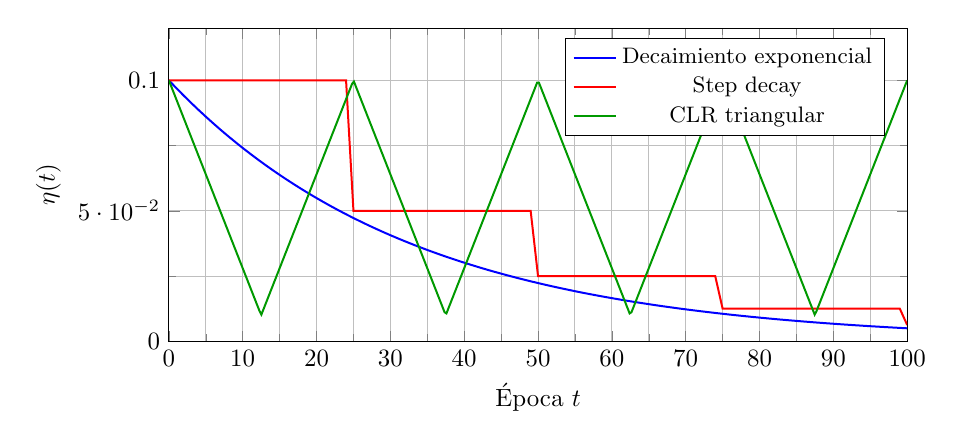
\begin{tikzpicture}[scale=0.9]
        \begin{axis}[
            width=12cm, height=6cm,
            xlabel={Época $t$},
            ylabel={$\eta(t)$},
            xmin=0, xmax=100,
            ymin=0, ymax=0.12,
            grid=both,
            minor tick num=1,
            legend pos=north east,
            legend style={font=\small}
        ]
            % Exponencial
            \addplot[blue, thick, domain=0:100, samples=101]
                {0.1 * exp(-0.03*x)};
            \addlegendentry{Decaimiento exponencial}
            % Step decay
            \addplot[red, thick, domain=0:100, samples=101]
                {0.1 * 0.5^(floor(x/25))};
            \addlegendentry{Step decay}
            % CLR triangular
            \addplot[green!60!black, thick, domain=0:100, samples=400]
                {0.01 + (0.1-0.01)*max(0, 1 - abs(x/25 - floor(x/25 + 0.5))*2)};
            \addlegendentry{CLR triangular}
        \end{axis}
    \end{tikzpicture}
    \caption{Comportamiento de tres heurísticas para la tasa de aprendizaje durante 100 épocas.}
    \label{fig:heuristicas-lr}
\end{figure}

La figura~\ref{fig:heuristicas-lr} ilustra cómo cada estrategia modifica la tasa a lo largo del entrenamiento. La elección depende del problema, pero en la práctica combinaciones como \emph{Adam con warm-up} o \emph{SGD con momentum + step decay} son estándares robustos.
